\chapter{Introduction}
\label{chapter:one}


Modern software systems nowadays provide configuration options to modify
both functional behavior of the system, i.e. functionality of the system, and non-functional properties of the system, such as performance and memory
consumption. 
Configuration options of a software system that are relevant to users are usually referred to as
features. All the features of a system (vector of configuration options) together defines a \textit{configuration} of a software system. The features can often taken integer, decimal or string values.  One of the most important non-functional properties is performance, because it  influences the how a user interacts with the system. 
Performance can be influenced by many factors including the environment (for example, the hardware in which the software system is current executing).  A software system is required to select and set configuration options to maximize the performance of that system. For example, say we have a software system with 10 (binary) configuration options---it results in a configuration space of size $2^{10}$ or $1024$. The user of the software system, now has to find the optimal configuration for the given task (or input) in hand. 
This problem can be tackled in two different ways: (1) exhaustively measuring performance of all possible configurations---which means running 1024 benchmark runs, and (2) use domain knowledge (assuming the user has tuned similar software system before) to find the best configuration. 
However, as the number of configuration options increase, it
becomes difficult for humans to keep track of the interactions between the configuration options. This means as the configuration space grows (size of the configuration space grows exponentially) it is harder to either exhaustively measure performance for all possible configurations or find domain experts to confidently do so. Please note that the optimal configuration we are trying to find can change dramatically with different inputs (tasks) and the environment---which make domain knowledge based decision less reliable. 

This exact problem has been reported by numerous researchers from different domains.
\begin{itemize}
\item Many software systems have poorly chosen defaults [1], [2]. Hence, it is useful to seek better configurations.
\item Understanding the configuration space of software systems with large configuration spaces is challenging [3].
\item Exploring more than just a handful of configurations is usually infeasible due to long benchmarking time [4].
\end{itemize}


The problem we are trying to tackle throughout this document is: "How can be find a set of configuration options which would \underline{maximize} the performance of a system while \underline{minimizing} the cost of search". Here were would limit our scope of study to just the configurations options or features of a particular software system (and not its environment). 

\begin{figure}[!htbp]
    \centering
    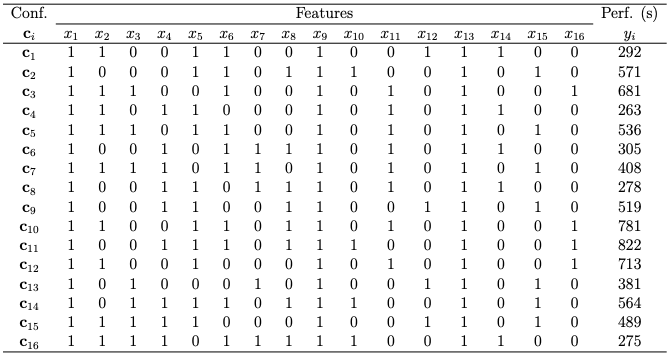
\includegraphics[width=0.8\linewidth]{Figures/table.png}
    \caption{A sample of 16 randomly-selected configurations of x264 and corresponding
performance measurements (seconds)}
    \label{fig:chap1_random_sample}
\end{figure}

\subsection{Motivating Example}
To motivate our work, we use the same example from our previous work citeGuoXXX, a configurable
command-line tool x264 for encoding video streams into the H.264/MPEG-4 AVC format.
In this example, we consider 16 encoder features of x264, such as encoding with multiple
reference frames and parallel encoding on multiple CPUs. The user can select
different features to encode a video. The encoding time is used to indicate the performance
of x264 in different configurations. A configuration represents a program variant with
a certain selection of features. This example with only 16 features gives rise to 1,152
configurations. Intuitively, 16 binary features should provide 216 different configurations,
however, in this work we consider only valid configurations i.e. configurations that are
allowed by the system under investigation.
In practice, often only a limited set of configurations can be measured, either by simulation
or by monitoring in the field. For example, Figure~\ref{fig:chap1_random_sample} lists a sample of 16 randomly selected
configurations and their actual performance measurements. How can we determine
the performance of other configurations based on a small random sample of measured configurations?
To formulate the above issue, we represent a feature as a binary decision variable x.
If a feature is selected in a configuration, then the corresponding variable is set to 1, and
0 otherwise. Assume that there are N features in total, all features of a program are
represented as a set X = {x1, x2, ..., xN }. A configuration is an N-tuple c, assigning 1 or 0
to each variable. For example, each configuration of x264 is represented by 16-tuple, e.g.
c1 = (x1 = 1, x2 = 1, x3 = 0, x4 = 0, ..., x16 = 1). All valid configurations of a program are
denoted by C.
Each configuration c of a program has an actual measured performance value y. Performance values are taken from publicly available dataset deployed with SPLConqueror
tool[17]. Detailed description of the dataset is given in Section 6.1.
All performance values of all configurations C form set Y . Suppose that we acquire a
random sample of configurations CS ? C and their actual measured performance values
YS ? Y , together forming sample S. The problem of variability-aware performance prediction
is to predict the performance of other configurations in C\CS based on the measured
sample S.
We regard all variables in X as predictors and a configuration?s actual performance
value y as the response. In other words, we predict a quantitative response y based on a
set of categorical predictors X, which is a typical regression problem[9]. Due to feature
interactions[18], the above issue is reduced to a non-linear regression problem, where the
response depends non-linearly on one or more predictors[8].












This dissertation is organized as follows.
Chapter~\ref{chapter:background} presents the background and related work.
Next, Chapter~\ref{chapter:inside-out} describes the design and implementation
of \emph{Inside-Out}, an approach to leverage low-level performance information
to achieve accurate and robust performance prediction.
In Chapter~\ref{chapter:cat}, we define cloud architecture tuning (CAT) and
describe its challenges.
We also discuss the state-of-the-art approaches and their pros and cons.
Chapter~\ref{chapter:arrow} proposes using low-level performance information
to enhance \bo, an online learning method to optimize any black-box function.
In Chapter~\ref{chapter:scout}, we design and implement \scout
, an efficient, effective and reliable CAT solution.
We also consider optimizing a group of workloads in Chapter~\ref{chapter:micky}.
In Chapter~\ref{chapter:dp}, we consider data placement to further optimize system performance.
Finally, Chapter~\ref{chapter:conclusion} concludes our discussion of cloud architecture tuning
and describes its future directions.
